\section{Virtual Heliodon}

	% Figures
	\begin{figure}[h]
	\centering
	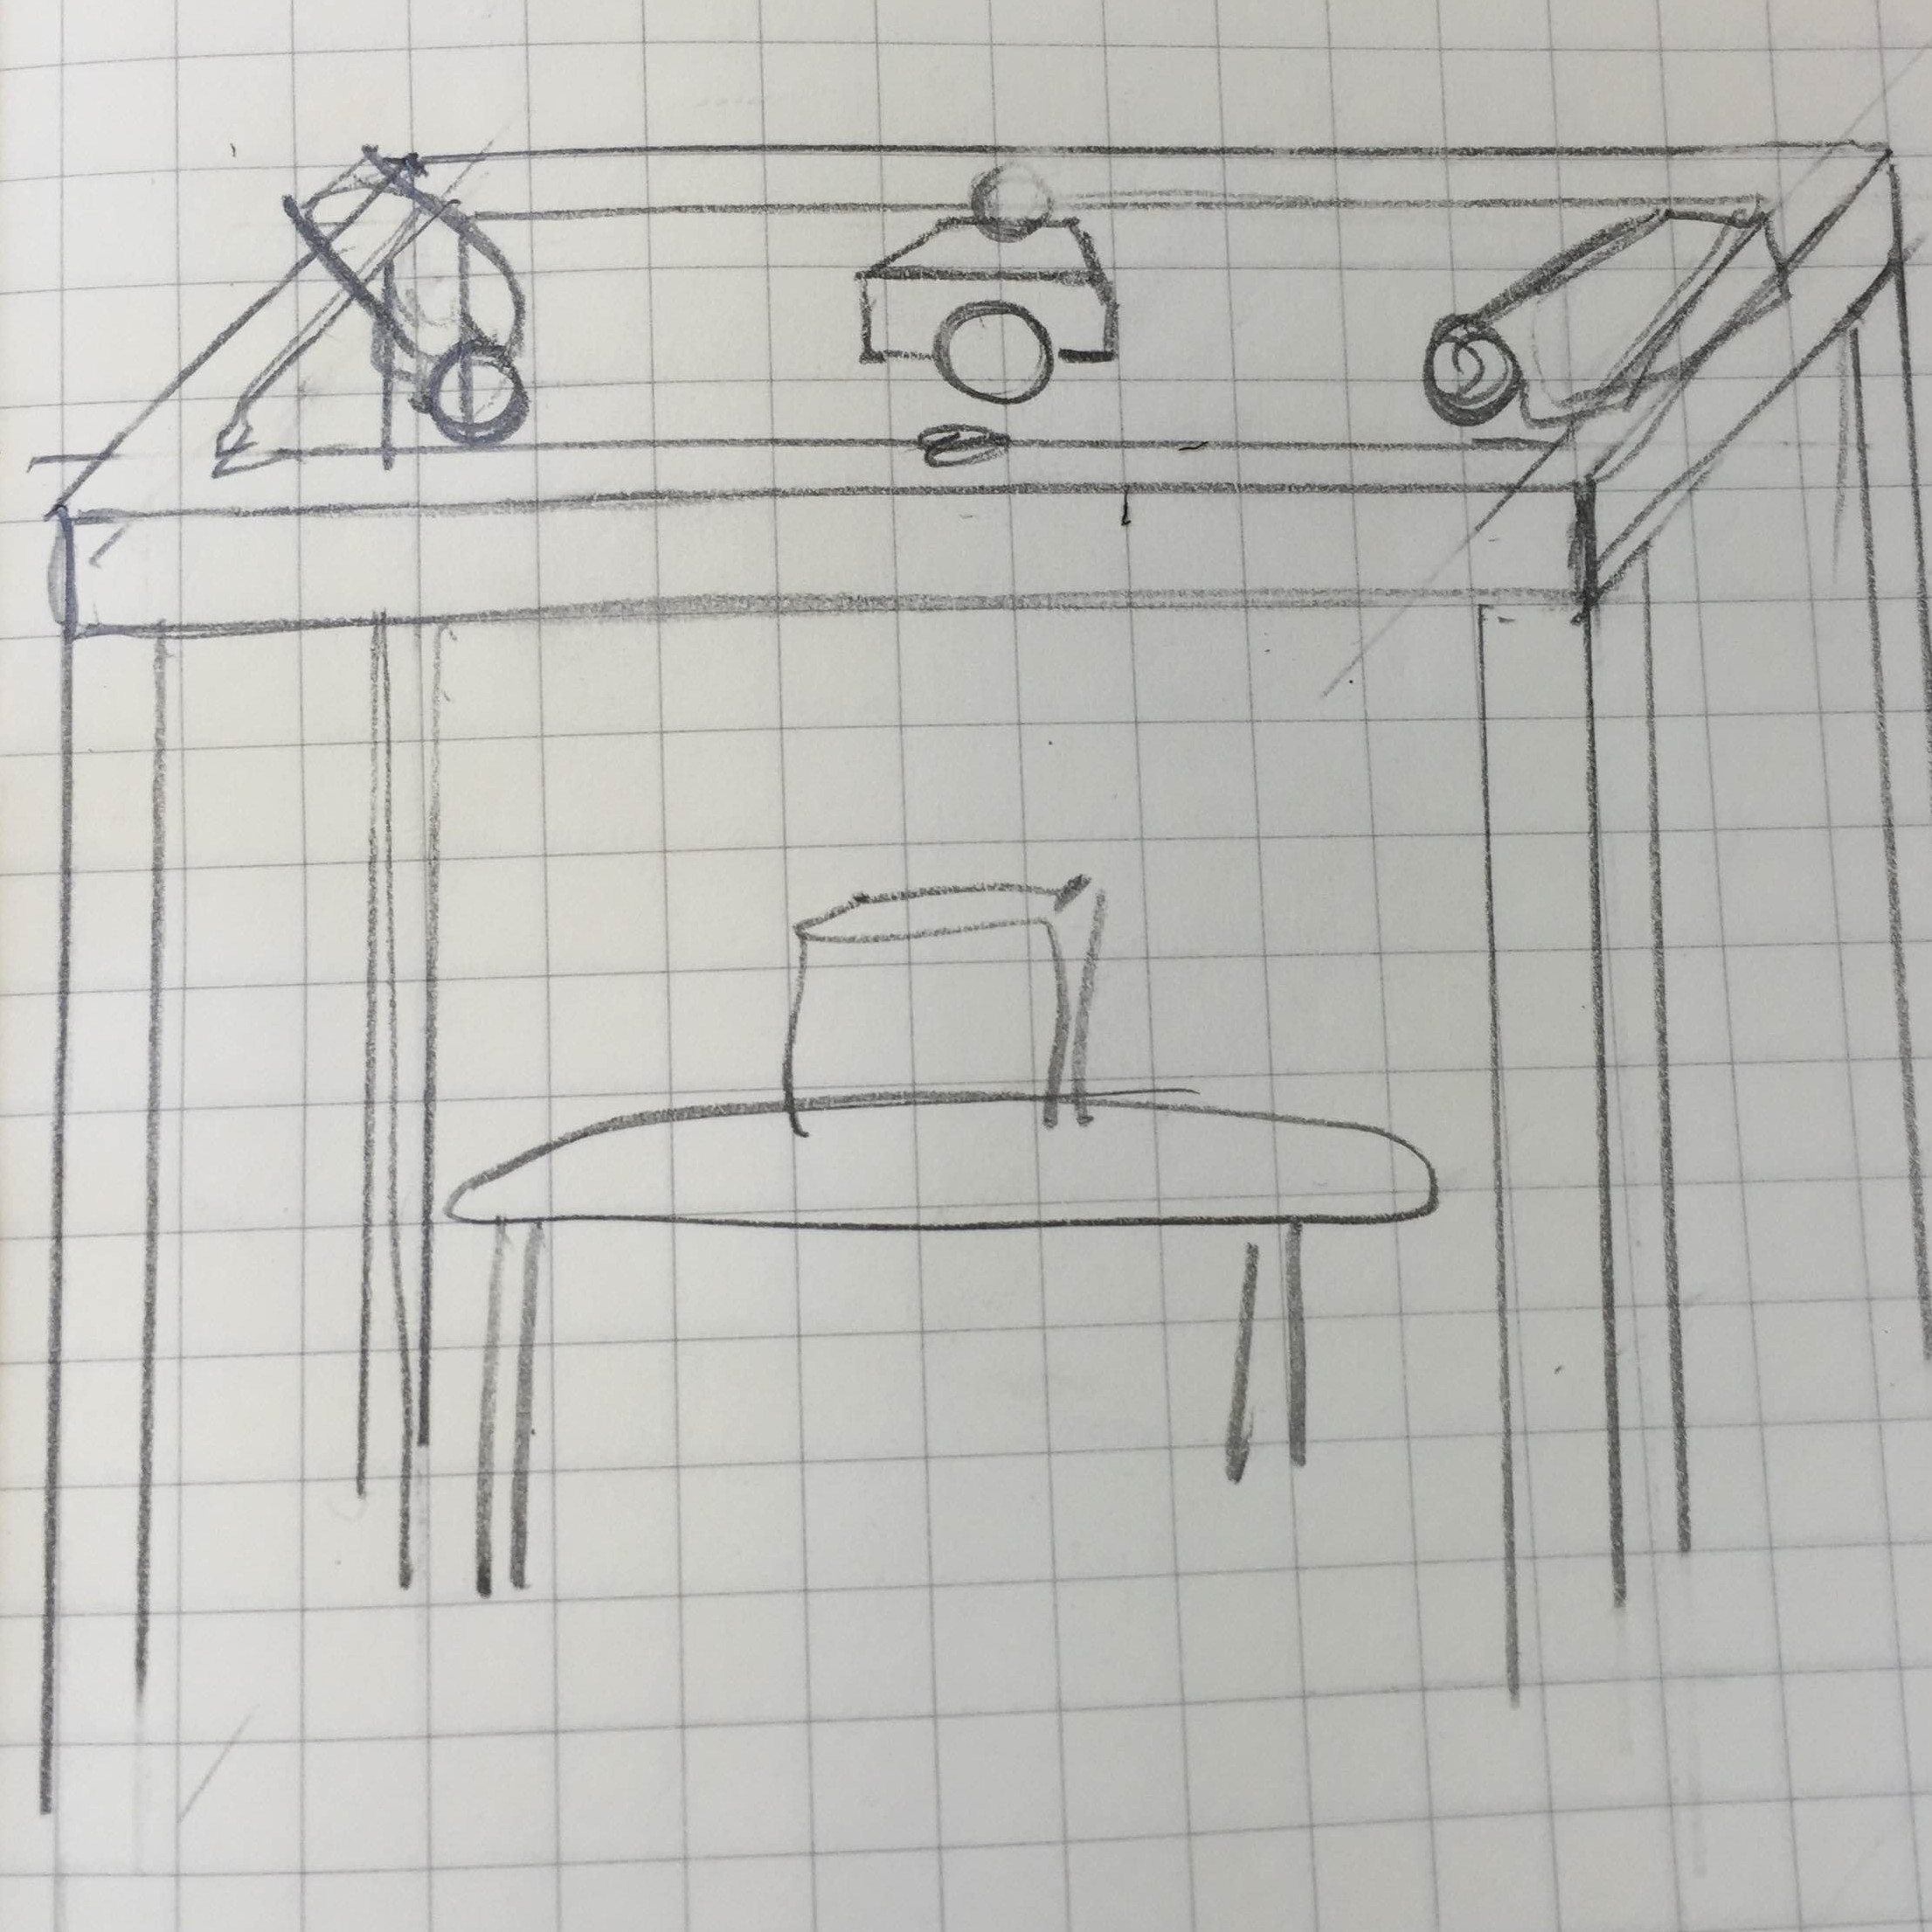
\includegraphics[width=0.5\textwidth]{virtual_heliodon}
	\label{fig:virtual_heliodon}
	\caption{Overview of the Virtual Heliodon. Note the projector arrangement and circle table at the center.}
	\end{figure}

	\begin{figure}[h]
	\centering
	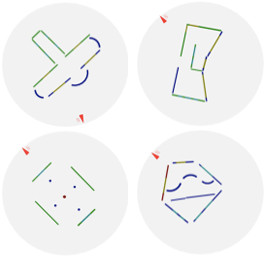
\includegraphics[width=0.5\textwidth]{heliodon_sketch}
	\label{fig:heliodon_sketch}
	\caption{Example physical sketches created by users on the Virtual Heliodon}
	\end{figure}

	The Virtual Heliodon is a spatial augmented reality with a tangible user interface for the early collaborative design of interior spaces with daylighting\cite{sheng2009virtual, cutler2009inferring,nasman2013physical,nasman2013evaluation,cutler2010interpreting}. 
	Succinctly, the Virtual Heliodon is composed of multiple projectors, a circular table, and a collection of foam primitives.  
	A large chassis holds the projectors above the table top at evenly spaced intervals. 
	These projectors all face towards the table top at the center of the system;
	The configuration of the Virtual Heliodon is shown below in figure-\ref{fig:virtual_heliodon}
	This tangible user interface lets users physically engage with wall primitives. 
	Users can define architectural spaces by moving and rotating wall primitives on the table top.
	Some architectural spaces created on the Virtual Heliodon are shown in figure-\cite{fig:heliodon_sketch}.
	Then a network of computers use the projectors to display daylighting simulation renderings onto the foam primitives placed on the table.
	In order to project on all wall primitives on the table top multiple projects in varying positions are used.
	Projecting daylighting rendering directly onto wall primitives creates an augmented reality environment that gives users a sense of immersion\cite{nasman2013evaluation}.
	The virtual Heliodon has gone through evaluations and has been proven to be engaging and valuable as an educational daylighting tool\cite{nasman2013evaluation}.

\section{Physical Sketch Interpretation Algorithm}

	Cutler et al. conducted evaluations on the effectiveness of physical sketch interpretation algorithm used in the Virtual Heliodon\cite{cutler2009inferring}.
	This studies compared user's intended interpretation of the physical sketches to both the algorithm's interpretation and other user's interpretation.
	In brief the study concluded that on average the physical sketch interpretation algorithm matched users intended interpretation 78\% of the time given non-ambiguous models\cite{cutler2009inferring}.
	Aside from ambiguous sketches, the Virtual Heliodon provided reliable 3D geometries that matched user's intended floor plan designs.
	OASIS uses the same physical sketching interpretation algorithm employed in the Virtual Heliodon.\\

	Interpreting sketches is not the only method of turning concepts into 3D models.
	Traditionally, both parametric and geometric modeling are used to create 3D models of architectural spaces.
	Daylighting analysis tools such as Home Energy Efficient Design tool(HEED) and eQuest use parametric modeling to generate 3D models of an architectural space\cite{hirsch2010equest,milne2001drag}.
	Parametric modeling is the creation of model from a template by specifying the parametric such as wall lengths, walls heights, and window positions through numerical entry.
	Both HEED and eQuest are intended for use in the schematic design phase and offer a large variety of energy analysis measures.
	Due to the high cost of effort in parametrically designing an architectural space, both HEED and eQUEST feature wizards to guide users through the process. 
	Geometric modeling is another modeling approach used by many architectural modeling software.
	SketchUp and AutoDesk are both popular architectural design tools that use geometric modeling for the generation of architectural spaces. 
	Geometric modeling gives users the ability to create 3D objects by modifying basic shapes visually; This modeling approach is similar to modeling with clay.
	The process of imagining a space and geometrically modelings that space in software is non-trivial.
	Being able to geometrically model complex 3D geometries is an art that requires precision and a deep understanding of the geometric tools available.
	As a result, the modeling of architectural designs in software is usually pushed back into the design development phase when fewer iterations a design are required\cite{Galasiu}.\\

	In practice, manual sketches are still used during the early design phase, because of the speed \& efficiently sketching offers designers\cite{Galasiu}.
	As a result researcher has been done on architectural sketching interfaces.
	LightSketch and the VR SketchPad project both incorporate architectural sketches into the early design phase\cite{do2001vr,glaser2003sketch}.
	Specifically, LightSketch shares much in common with OASIS.
	LightSketch gives users the ability to to draw walls, windows, and interior lighting elements to define architectural spaces\cite{glaser2003sketch}; The drawings are interpreted and turned into 3D models.
	Users can then perform daylighting analysis and generate renderings from generated 3D models.
	LightSketch, however, is limited to shoe-box geometries for rooms.
	Users cannot freely design a wide variety of non shoe-box of floor plans as is possible in the VR SketchPad project and the Virtual Heliodon.
	The VR SketchPad project supports the creation of 3D models of a wide variety of architectural spaces\cite{do2001vr}.
	Furthermore the VR Sketchpad was available as an online tool, similar to OASIS.
	The VR SketchPad project however does not distinguish between interior and exterior spaces but instead just renders objects where users sketch them.
	Sketches in the Virtual Heliodon get converted into water-tight models that are required for daylighting simulations.\\

\section{Daylighting Render LSVO}

	In addition to using the Virtual Heliodon's physical sketch interpretation algorithm, I use the Virtual Heliodon's GPU photon mapping rendering engine\cite{li2011photon,nasman2013physical}. 
	This rendering engine is specialized to provide viewpoint independent daylight renderings at interactive rates.
	The Virtual Heliodon's rendering engine takes advantage of NVidia's Optix GPU ray tracing framework for the parallelization of photon mapping\cite{parker2010optix}.
	Concisely, photon mapping is the approximation of global illumination by tracing rays outward from emitters and then gathering photons after several bounces to calculate indirect illumination per triangle or patch\cite{hachisuka2008progressive}.
	When photons leave emitters their position and direction are chosen at random, however, a photon's intensity is a function of its direction as defined by the International Commission on Illumination's sky models\cite{de1994spatial}. 
	Other daylighting renderer, such as Radiance require more time to produce clear and noise-free results\cite{compagnon1997radiance}. 
	However, Radiance is validated and a result Radiance is widely used as a back-end component to several daylighting tools\cite{reinhart2006development, Galasiu}.
	While, the Virtual Heliodon's rendering engine has not been directly validated against Radiance, the rendering engine has been validated against a radiosity based render.
	This radiosity based renderer, used in previous versions of the Virtual Heliodon, was validated against Radiance\cite{sheng2010global}. 
	In brief, the Virtual Heliodon's rendering engine serves our needs as a fast renderer for qualitative analysis during the early stages of design.

\section{Related Software}

	OASIS shares goals in common with many other daylighting analysis software.
	Increased value on sustainability and energy efficiency drives the development of simple analysis tools for use in the early design phase of the architectural design processes.
	One such piece of software is AutoDesk's latest early design tool, Project Vasari\cite{vasari,autodesk}.
	Project Vasari is a stand alone geometric modeling tool with a similar interface as AuthoDesk's Revit\cite{revit}.
	Project Vasari, unlike Revit, was designed for energy analysis during the conceptual design of architectural spaces. 
	As a result, Project Vasari comes packaged with win. client, daylighting, and whole building energy analysis visualizations.
	Another tool with similar features is Ecotect -- an AutoDesk plug in\cite{ecotect}.
	Ecotect offers a collection of useful visualizations such as sun paths, previews of building shadows, and daylighting factor visuals.
	SketchUp is another notable conceptual design tool\cite{sketchup}. 
	Although SketchUp does not directly support energy analysis and advance daylighting features, there are a handful of plug ins that do.
	for example VE-Ware by IES is a free energy and carbon plug in for SketchUp and Revit\cite{veware}. 
	VE-Ware, given a model created in SketchUp will generate detailed energy analysis reports. Generally, energy analysis plug ins that support daylighting  measurements, exist for most major architectural modeling softwares.
	For instance, Rhinoceros, as general 3D Modeling tool commonly used for creating architectural models, supports plugs in such as LadyBug  for basic energy analysis\cite{rhino,ladybug}. 
	Also, another noteworthy extension to SketchUp includes Lightsolve\cite{andersen2008intuitive}.
	While Lightsolve is not officially a SketchUP plug in, it does support importing models directly from SketchUp.
	LightSolve is noteworthy because the tool's main focus is on daylighting analysis.
	Anderson et al. developed Lightsolve as an early design daylighting analysis tool that gives designers not only annual metrics but also qualitative renderings of their designs. 
	Within the application designers could analyze both quantitative illumination metrics of particular locations in a design but also view renderings of those locations from multiple viewpoints.
	Lightsolve also provides visual sun positions and elevation information on the same page as the daylighting metrics and renderings. 
	All of these visual elements on the same display offers designers a better understanding of daylighting conditions within their designed architectural spaces\cite{andersen2011informing}. 
	On the whole, all of these tools offer rich and informative daylighting analysis during the conceptual  design of architectural spaces.
	However they all in some way rely on geometrically created models.
	During the conceptual/early design stages of architectural design, the ability to express concepts ad 3D models quickly is invaluable.
	As a result , researchers have investigated faster and more initiatives ways to generate 3D models for daylighting analysis.
